%!TEX root = ../dissertation.tex

\chapter{Evaluation}
\label{chapter:evaluation}

The success of a software system is often dependent on the opinion of the people that will use it. Systems attractive and easy to use according to the target audience background are more likely to be highly used.

The developed system tries to make the task of reading, understanding and structuring a software description article into an easy one, providing a simple and clean interface.

As the main goal of the developed application is to be used by students and teachers, in both classroom and home environments, it was asked to the students enrolled in the Software Architectures course to test the application, namely the features for annotating text and structuring Scenarios from the annotations created.

The participating students were asked to fill a small survey afterwards to register their opinions.
This survey consisted of a grid question to evaluate aspects of the application usability in a scale from one to ten, three questions asking to evaluate the usefulness of the application in a scale of one to ten, and three open and optional questions, asking what did the student like the most about the application, what improvements could be done to it, and to register any other feedback the student may had.

A total of eight students volunteered to test the application. From these eight, four answered the survey. Due to the small number of participants and little feedback, the results shown are merely indicative, as it is impossible to take valuable conclusions from such a small sample.

Regarding the usability of the application, Figure \ref{figure:usabilityEvaluation} shows the graph containing the ratings given by the students.

\begin{figure}[h]
\centering
\begin{normalsize}
\textbf{Usability of the Application's Features}\\
\end{normalsize}
\scriptsize
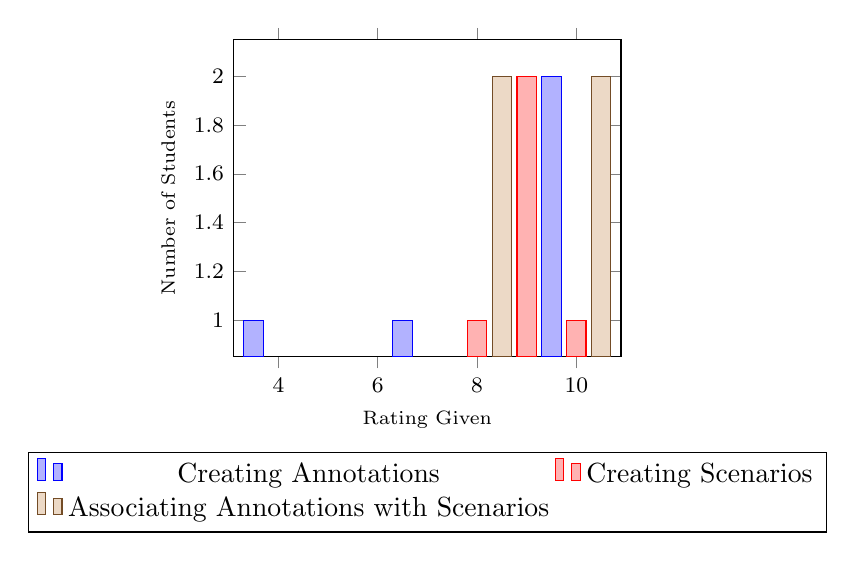
\begin{tikzpicture}
\begin{axis}[
small,
x tick label style={
/pgf/number format/1000 sep=},
ylabel=Number of Students,
ylabel style={font=\scriptsize},
xlabel=Rating Given,
xlabel style={font=\scriptsize},
enlargelimits=0.15,
legend style={at={(0.5,-0.3)},
anchor=north,legend columns=2},
ybar,
bar width=7pt,
]
\addplot 
	coordinates {(7,1) (4,1) (10,2)};
\addplot 
	coordinates {(9,2) (10,1) (8,1)};
\addplot
	coordinates {(8,2) (10,2)};		
\legend{Creating Annotations, Creating Scenarios, Associating Annotations with Scenarios}
\end{axis}
\end{tikzpicture}
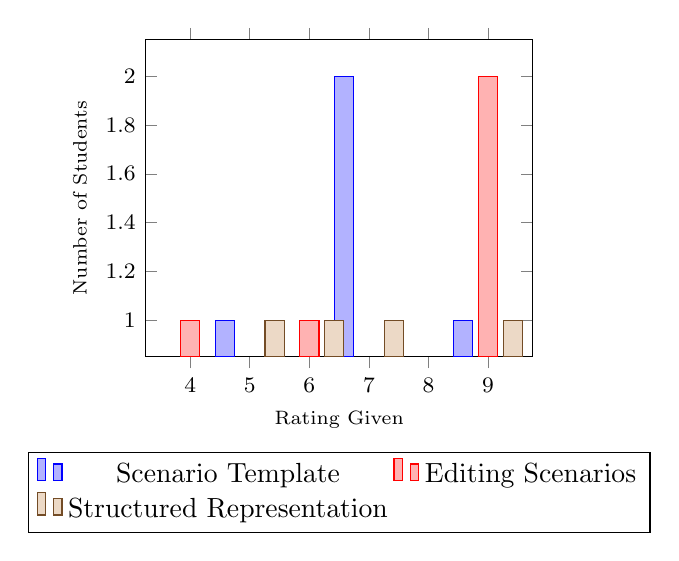
\begin{tikzpicture}
\begin{axis}[
small,
x tick label style={
/pgf/number format/1000 sep=},
ylabel=Number of Students,
ylabel style={font=\scriptsize},
xlabel=Rating Given,
xlabel style={font=\scriptsize},
enlargelimits=0.15,
legend style={at={(0.5,-0.3)},
anchor=north,legend columns=2},
ybar,
bar width=7pt,
]

\addplot
	coordinates {(5,1) (7,2) (9,1)};
\addplot
	coordinates {(4,1) (6,1) (9,2)};
\addplot
	coordinates {(5,1) (6,1) (9,1) (7,1)}; 	
\legend{Scenario Template, Editing Scenarios, Structured Representation}
\end{axis}
\end{tikzpicture}
\caption{Evaluation results regarding the usability of the application}
\label{figure:usabilityEvaluation}
\end{figure}

Overall students thought the application is easy to use regarding creating Scenarios and associating annotations with them. However, there were complaints about the AnnotatorJS interface, such as ``I had trouble when trying annotate a sequence of letters when that sequence overlapped with another annotation'', which implies that it is not very intuitive when trying to create multiple annotations in the same piece of text.

Improvements suggested in the survey include \textit{``There should be a way to ``view'' the scenario itself, with the diagram that is showed in the lectures. Also, the system needs to be more intuitive, particularly when it comes to selecting sentences for the scenarios''} and \textit{``Make multiple copies of the article to be only seen by each group so that one group doesn't get confused or get influenced by others.''}. This reinforces the idea that the AnnotatorJS interface is not very intuitive sometimes, and the need of creating groups in the platform, which is explained in \ref{chapter:futureWork}.

When asked what did they like the most about the application, students pointed that ``It is possible for different people to analyze the same document, and its easy to use'' and ``It provides a quick and convenient way of constructing scenarios''. These opinions help conclude that the platform satisfies the requirement of providing collaboration among students, and facilitates understanding the Software Architectures concepts.

Regarding the usefulness of the application, the survey asked to rate how much the application facilitates the application of theoretical concepts to practical examples, and how useful would it be in the context of the Group Assignments and Practical Classes. Figure \ref{figure:usefulnessEvaluation}

\begin{figure}[h]
\centering
\begin{normalsize}
\textbf{Application Usefulness}\\
\end{normalsize}
\scriptsize
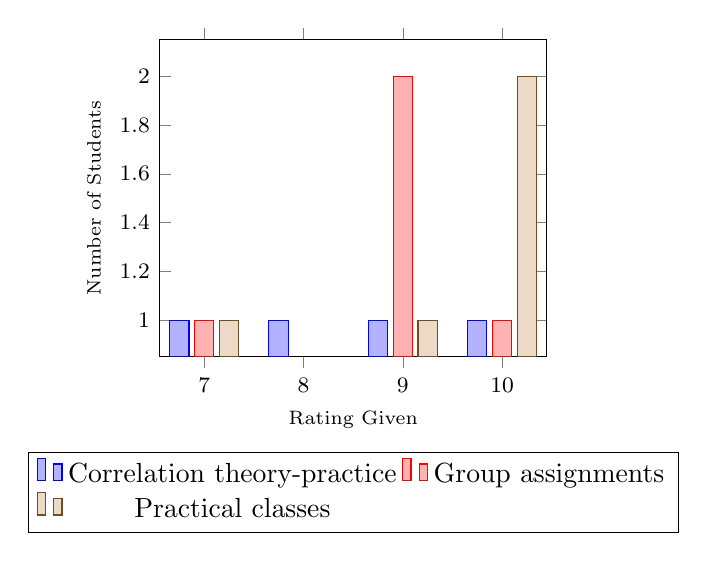
\begin{tikzpicture}
\begin{axis}[
small,
x tick label style={
/pgf/number format/1000 sep=},
ylabel=Number of Students,
ylabel style={font=\scriptsize},
xlabel=Rating Given,
xlabel style={font=\scriptsize},
enlargelimits=0.15,
legend style={at={(0.5,-0.3)},
anchor=north,legend columns=2},
ybar,
bar width=7pt,
]
\addplot 
	coordinates {(7,1) (8,1) (9,1) (10,1)};
\addplot 
	coordinates {(9,2) (7,1) (10,1)};
\addplot
	coordinates {(7,1) (9,1) (10,2)};		
\legend{Correlation theory-practice, Group assignments, Practical classes}
\end{axis}
\end{tikzpicture}
\caption{Evaluation of the usefulness of the application}
\label{figure:usefulnessEvaluation}
\end{figure}

Overall, students would like to use this application for both their Group Assignments and when discussing a description article in the Practical classes. 

In conclusion, the evaluation of the platform, despite the small number of testers, provided positive feedback. The platform proved to provide collaboration, and students appreciated how the information from the text can be extracted into a single template. 
